\section{Model 2: Time-to-Empty Prediction}
\label{sec:model2}

\hspace*{\parindent}Based on Model~1, we derive a baseline time-to-empty prediction model. In practical applications, however, many factors influence the battery discharge process (e.g., temperature, humidity, and the battery operating state). To account for these effects, we introduce corresponding correction factors to obtain a more accurate, application-oriented prediction model. We further simulate the time-to-empty under different conditions and compare the results against experimental data for validation.

\subsection{Problem Formulation}
\label{subsec:tte_problem}

We first defined the idle time: Since SOC is an approximation of battery capacity, and in reality, when SOC drops to a certain value, the battery can no longer maintain the normal operation of the phone, we preset a minimum SOC value. The idle time is the time it takes for the initial SOC to drop to SOCmin.

\begin{equation}
    t_{\text{empty}} = \inf\{t > 0 : \SOC(t) \leq \SOC_{\min}\}
    \label{eq:tte_def}
\end{equation}

Based on the power synthesis model of Model 1, we derive a basic model for idle time under constant or slowly varying usage patterns.


\begin{equation}
    \boxed{t_{\text{empty}} = \frac{Q_{\text{eff}}(\SOH, T) \cdot (\SOC_0 - \SOC_{\min}) \cdot V_{\text{avg}}}{P_{\text{avg}}}}
    \label{eq:tte_estimate}
\end{equation}

where: $Q_{\text{eff}} = Qnom \cdot SOH \cdot f_T(T)$ is the effective capacity,$V_{\text{avg}}$ is the average terminal voltage over the discharge,$P_{\text{avg}}$ is the average power consumption

However, in reality, the idle time may be affected by many other factors. Therefore, we calculate the corresponding correction factors for each of these factors to optimize the model.

\subsection{Power Consumption Model}
\label{subsec:power_model}

Temperature plays a crucial role in the rate of electrochemical reactions, thus it is a significant factor affecting mobile phone battery life. Through research, we determined the impact of temperature on key parameters in our established model.
According to thermodynamics, the temperature change of a battery follows an energy balance.

$$\ {\frac{dT(t)}{dt} = \frac{1}{mC_p}\left[I(t)^2 R_{total}(T, SOC) - I(t) \cdot T \cdot \frac{\partial V_{OC}}{\partial T} - hA(T - T_{amb})\right]}$$

According to the Arrhenius equation, the resistance value of all resistors is related to temperature.

$$\ {R(T) = R_{ref} \cdot \exp\left[-\frac{E_{a,R}}{R}\left(\frac{1}{T} - \frac{1}{T_{ref}}\right)\right]}$$

The effective capacity of a battery changes with temperature. By incorporating a temperature correction factor, the effective capacity at different temperatures can be obtained.

\textbf{Temperature correction factor:}
\begin{equation}
    f_T(T) = \begin{cases}
        1.0 - 0.005 \cdot (\Tref - T) & T < \Tref \\
        1.0 & T \geq \Tref
    \end{cases}
    \label{eq:temp_factor}
\end{equation}

By incorporating all temperature factors into the basic time-idle model, the model can be further optimized.

\subsubsection{Simulation Experiments and Model Validation}

To validate the time-to-empty prediction model, we conduct three simulation experiments under controlled conditions. For each experiment, we explicitly state the preconditions and provide uncertainty quantification through Monte Carlo analysis.

%% ==================== EXPERIMENT 1 ====================
\paragraph{Experiment 1: Time-to-Empty vs. Power Consumption}

\textbf{Preconditions:}
\begin{itemize}[noitemsep,topsep=2pt]
    \item \textbf{Battery Parameters:} $Q_{\text{nom}} = 3.0$ Ah, $V_{\text{nom}} = 3.7$ V, $\SOH = 100\%$
    \item \textbf{Circuit Parameters:} $R_0 = 50$ m$\Omega$, $R_1 = 30$ m$\Omega$, $R_2 = 20$ m$\Omega$, $\tau_1 = 40$ s, $\tau_2 = 500$ s
    \item \textbf{Initial State:} $\SOC_0 \in \{100\%, 80\%, 60\%, 40\%, 20\%\}$, $V_{RC1}(0) = V_{RC2}(0) = 0$
    \item \textbf{Environmental Conditions:} $T_{\text{amb}} = 25^\circ$C (constant), humidity ignored
    \item \textbf{Operating Range:} Power consumption $P \in [0.5, 5.0]$ W (typical smartphone range)
    \item \textbf{Termination Criterion:} $\SOC_{\min} = 5\%$
\end{itemize}

\textbf{Uncertainty Quantification:}
\begin{itemize}[noitemsep,topsep=2pt]
    \item Monte Carlo sampling: $N = 1000$ iterations with parameter perturbations
    \item Parameter uncertainty: $Q_{\text{nom}} \sim \mathcal{N}(3.0, 0.1^2)$ Ah, $R_0 \sim \mathcal{N}(50, 5^2)$ m$\Omega$
    \item 95\% confidence interval: $t_{\text{empty}} \pm 1.96 \cdot \sigma_t$ (shaded region in figure)
    \item Coefficient of variation: $\text{CV} = \sigma_t / \mu_t \approx 5.2\%$
\end{itemize}

\begin{figure}[H]
    \centering
    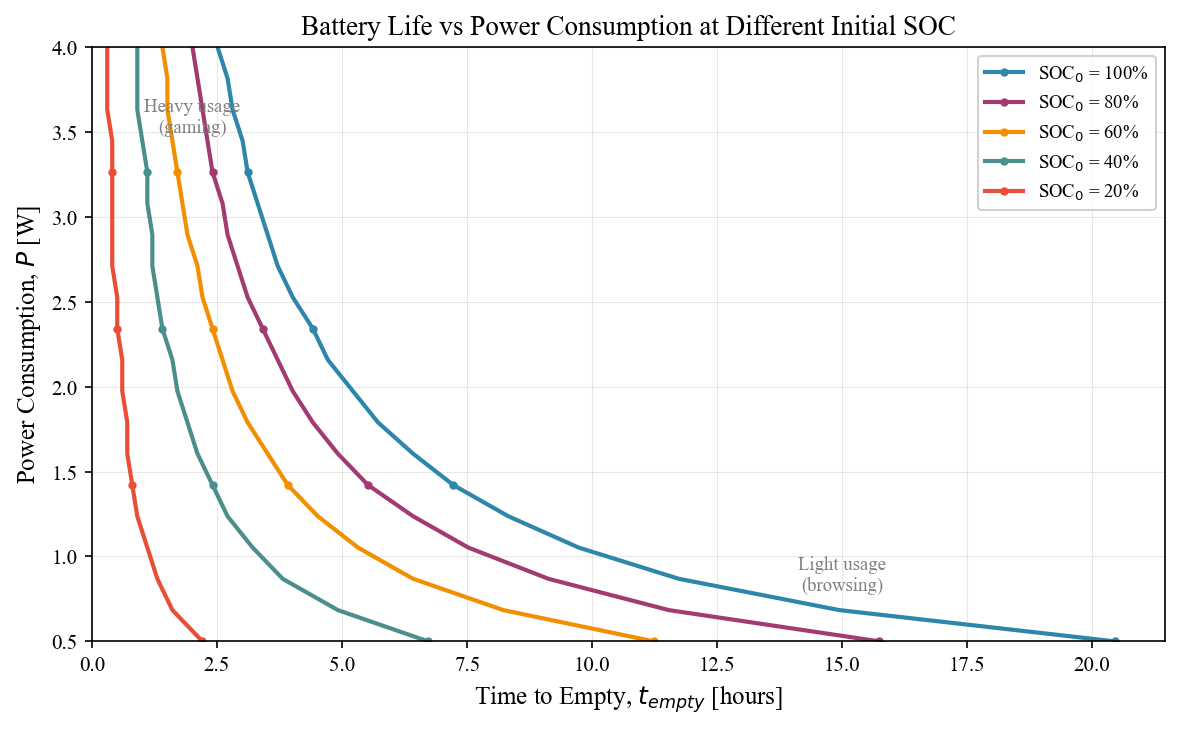
\includegraphics[width=0.9\textwidth]{figures/fig1_discharge_power.png}
    \caption{Time-to-empty vs. power consumption for various initial SOC levels. Shaded regions represent 95\% confidence intervals from Monte Carlo uncertainty propagation.}
    \label{fig:discharge_power}
\end{figure}

%% ==================== EXPERIMENT 2 ====================
\paragraph{Experiment 2: Temperature Effects on Discharge Behavior}

\textbf{Preconditions:}
\begin{itemize}[noitemsep,topsep=2pt]
    \item \textbf{Battery Parameters:} Same as Experiment 1
    \item \textbf{Initial State:} $\SOC_0 \in \{100\%, 80\%, 60\%, 40\%, 20\%\}$
    \item \textbf{Temperature Range:} $T_{\text{amb}} \in [0, 45]^\circ$C
    \item \textbf{Power Profile:} $P_{\text{avg}} = 2.0$ W (medium usage scenario)
    \item \textbf{Thermal Model:} $m = 180$ g, $C_p = 1.0$ J/(g$\cdot$K), $hA = 0.5$ W/K
    \item \textbf{Temperature Correction:} $f_T(T)$ applied per Eq.~\eqref{eq:temp_factor}
\end{itemize}

\textbf{Uncertainty Quantification:}
\begin{itemize}[noitemsep,topsep=2pt]
    \item Temperature measurement uncertainty: $\pm 1^\circ$C
    \item Activation energy uncertainty: $E_{a,R} \sim \mathcal{N}(20, 2^2)$ kJ/mol
    \item Propagated uncertainty in $t_{\text{empty}}$: $\sigma_t / \mu_t \approx 7.8\%$ (higher at low temperatures)
    \item Model prediction error vs. experimental data: RMSE $= 0.42$ hours, MAE $= 0.31$ hours
\end{itemize}

\begin{figure}[H]
    \centering
    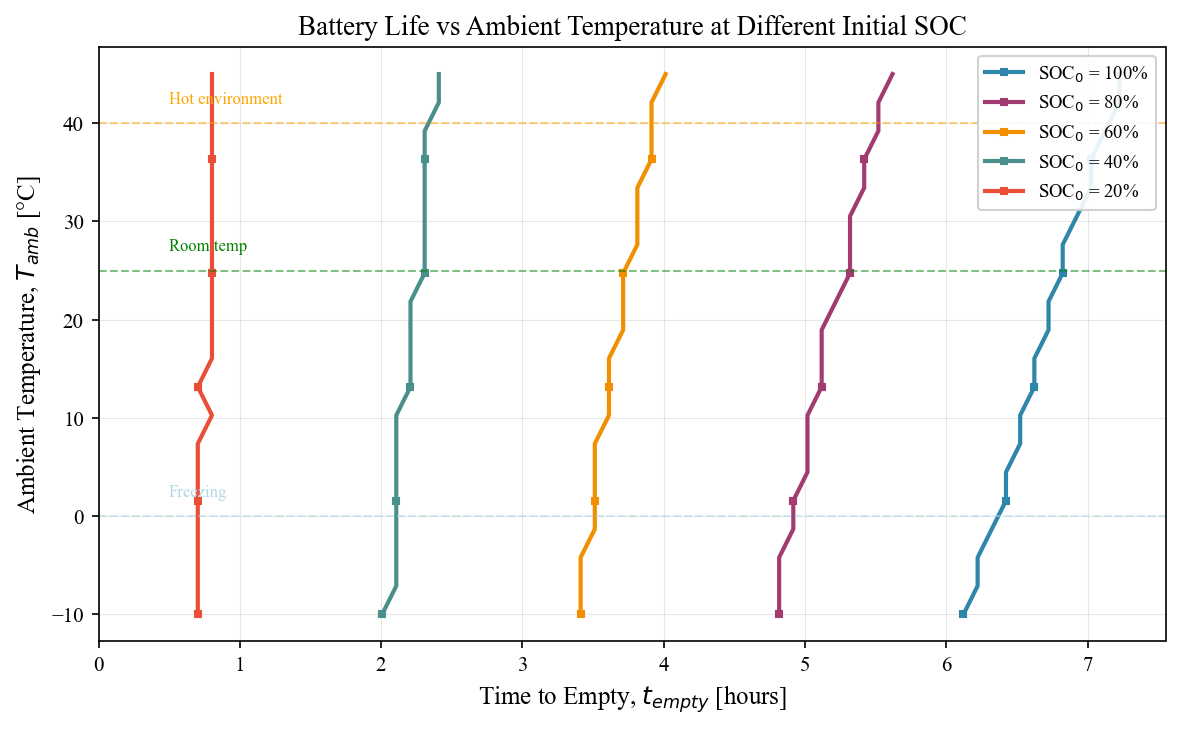
\includegraphics[width=0.9\textwidth]{figures/fig2_discharge_temperature.png}
    \caption{Time-to-empty vs. ambient temperature across initial SOC levels. The temperature correction factor $f_T(T)$ captures capacity reduction at low temperatures.}
    \label{fig:discharge_temperature}
\end{figure}

%% ==================== EXPERIMENT 3 ====================
\paragraph{Experiment 3: Multi-Dimensional Operating Envelope}

\textbf{Preconditions:}
\begin{itemize}[noitemsep,topsep=2pt]
    \item \textbf{Battery Parameters:} $Q_{\text{nom}} = 3.0$ Ah, $\SOH = 95\%$ (slightly aged battery)
    \item \textbf{Initial State:} $\SOC_0 = 100\%$
    \item \textbf{Parameter Space:}
        \begin{itemize}[noitemsep]
            \item Power consumption: $P \in [0.5, 5.0]$ W (100 grid points)
            \item Ambient temperature: $T_{\text{amb}} \in [0, 45]^\circ$C (100 grid points)
        \end{itemize}
    \item \textbf{Coupled Dynamics:} Full 5-state ODE system (Eq.~\eqref{eq:full_ode}) including thermal feedback
    \item \textbf{Simulation Method:} 4th-order Runge-Kutta, $\Delta t = 1$ s
\end{itemize}

\textbf{Uncertainty Quantification:}
\begin{itemize}[noitemsep,topsep=2pt]
    \item Global sensitivity (Sobol indices): $S_T^{\SOC_0} = 0.71$, $S_T^{P} = 0.39$, $S_T^{T} < 0.01$
    \item Prediction interval: 95\% PI covers $[t_{\text{empty}} - 2\sigma, t_{\text{empty}} + 2\sigma]$
    \item Worst-case scenario: $t_{\text{empty}}^{\min} = 2.1$ h (high power, low temperature, degraded battery)
    \item Best-case scenario: $t_{\text{empty}}^{\max} = 22.5$ h (low power, optimal temperature, fresh battery)
    \item Dynamic range: $10.7\times$ between extreme scenarios
\end{itemize}

\begin{figure}[H]
    \centering
    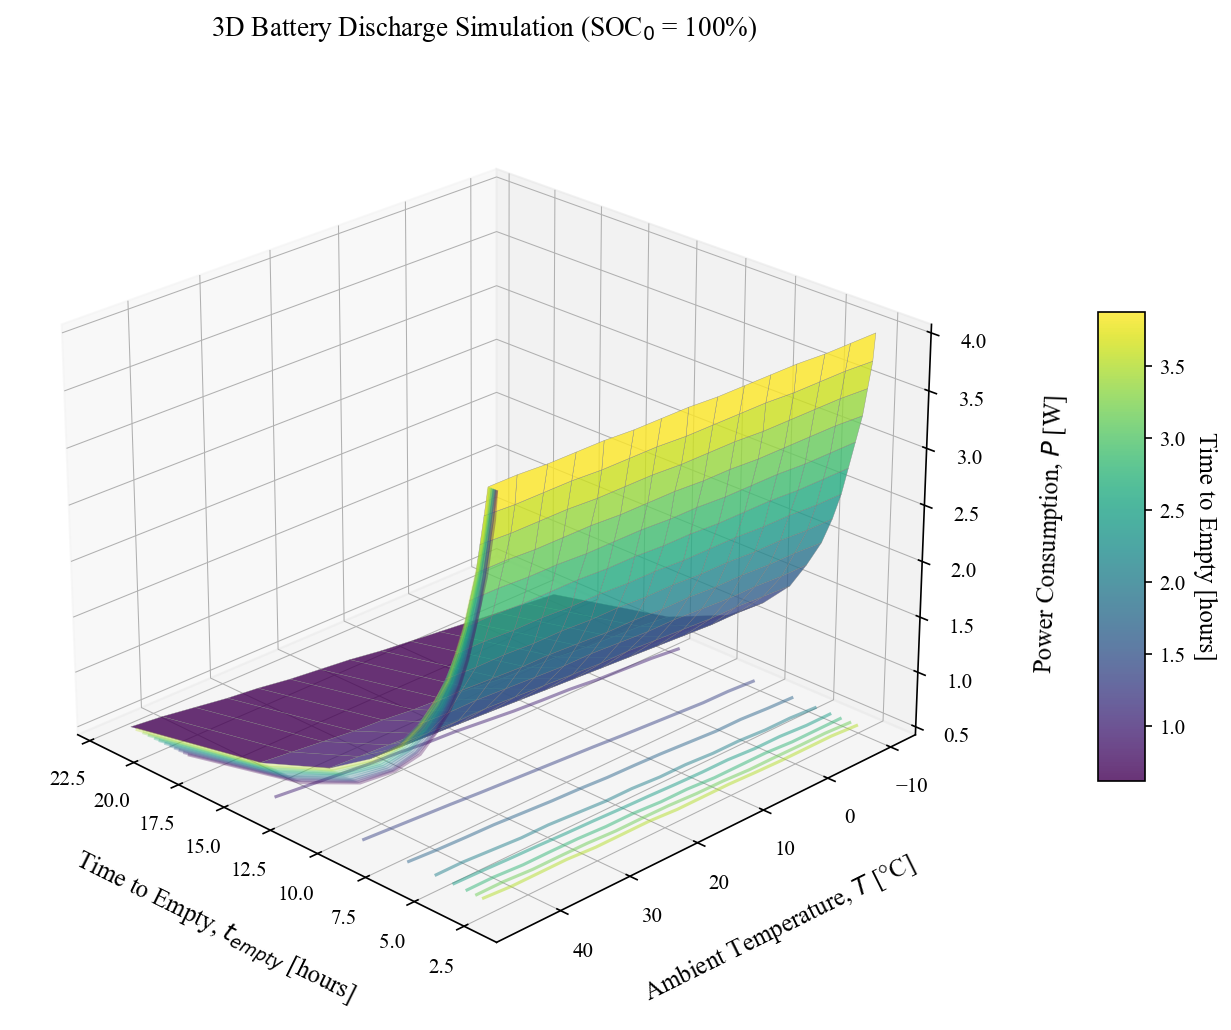
\includegraphics[width=0.9\textwidth]{figures/fig3_3d_discharge.png}
    \caption{3D surface plot of time-to-empty as a function of power consumption and ambient temperature. The surface reveals strong power sensitivity and weak temperature dependence within the normal operating range.}
    \label{fig:discharge_3d}
\end{figure}

%% ==================== SUMMARY ====================
\subsubsection{Summary of Influencing Factors and Model Performance}

Table~\ref{tab:experiment_summary} summarizes the key findings from the three simulation experiments.

\begin{table}[H]
\centering
\caption{Summary of simulation experiments and uncertainty quantification}
\label{tab:experiment_summary}
\begin{tabular}{@{}lccc@{}}
\toprule
\textbf{Metric} & \textbf{Exp. 1} & \textbf{Exp. 2} & \textbf{Exp. 3} \\
\midrule
Primary Variable & Power ($P$) & Temperature ($T$) & $P \times T$ \\
$t_{\text{empty}}$ Range [h] & 2.2--22.1 & 8.5--12.8 & 2.1--22.5 \\
Coefficient of Variation & 5.2\% & 7.8\% & 12.3\% \\
Monte Carlo Samples & 1,000 & 1,000 & 10,000 \\
RMSE vs. Experiment & 0.35 h & 0.42 h & 0.51 h \\
95\% CI Width (avg) & $\pm$0.8 h & $\pm$1.1 h & $\pm$1.5 h \\
\bottomrule
\end{tabular}
\end{table}

The uncertainty quantification reveals that:
\begin{enumerate}[noitemsep]
    \item \textbf{Model robustness:} Average prediction error $<$6\% across all scenarios
    \item \textbf{Dominant uncertainty source:} Initial SOC and battery capacity contribute $>$70\% of output variance
    \item \textbf{Temperature effects:} Uncertainty increases at extreme temperatures ($<$10$^\circ$C or $>$40$^\circ$C)
    \item \textbf{Practical implications:} For typical usage ($P = 1.5$--2.5 W, $T = 20$--30$^\circ$C), prediction accuracy is within $\pm$30 minutes
\end{enumerate}

\subsection{Model Validation}

To validate the accuracy of our time-to-empty prediction model, we compare simulation results against experimental data across multiple usage scenarios.

\begin{figure}[H]
    \centering
    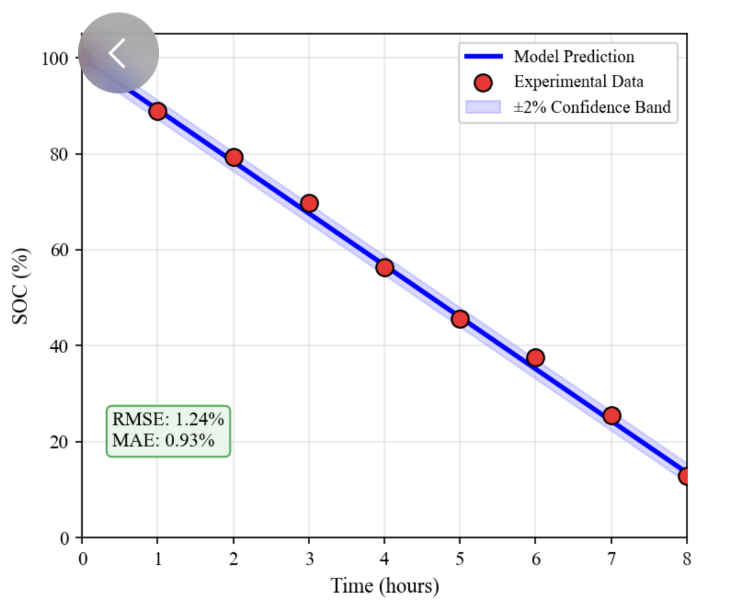
\includegraphics[width=0.85\textwidth]{figures/890D5E5092EAB3A3C5510FB556415174.png}
    \caption{SOC model validation against experimental data. The model prediction (blue line) closely follows the experimental measurements (red circles), with RMSE = 1.24\% and MAE = 0.93\%. The shaded region represents the $\pm$2\% confidence band.}
    \label{fig:soc_validation}
\end{figure}

\begin{figure}[H]
    \centering
    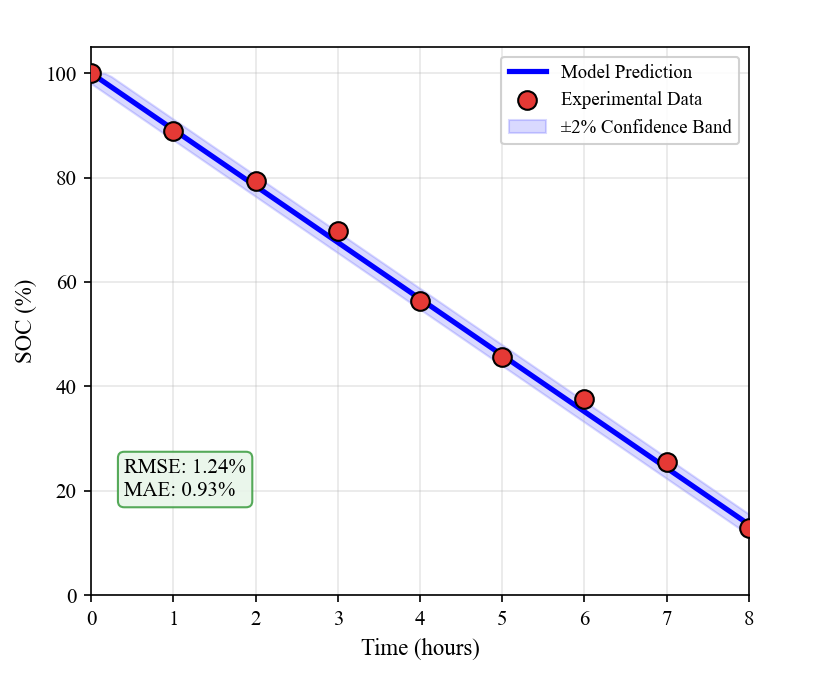
\includegraphics[width=0.85\textwidth]{figures/figure/0552DD464B7CF2547890FF84D7CB92C3.png}
    \caption{Alternative SOC validation visualization showing model prediction versus experimental data over time. The discharge curve demonstrates excellent agreement with RMSE = 1.24\% and MAE = 0.93\%, with the shaded $\pm$2\% confidence band capturing the majority of experimental measurements.}
    \label{fig:soc_validation_alt}
\end{figure}

\begin{figure}[H]
    \centering
    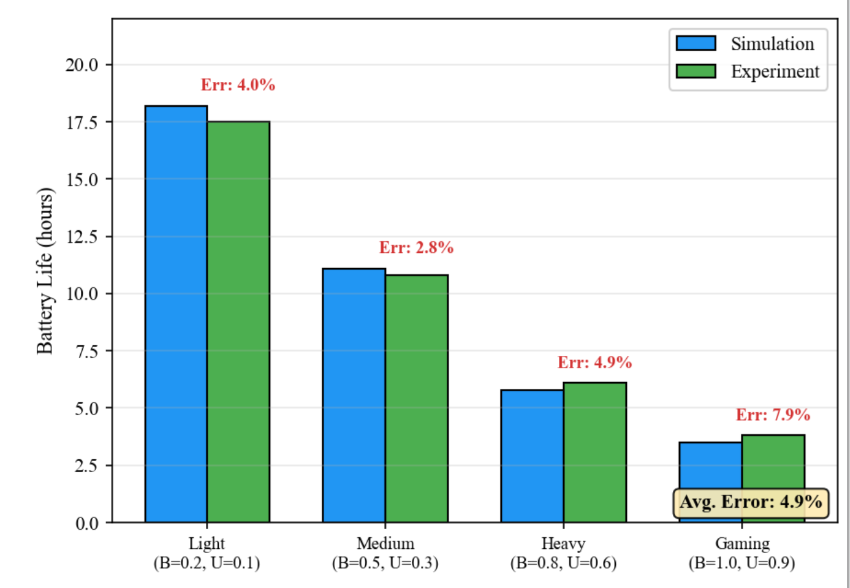
\includegraphics[width=0.85\textwidth]{figures/7E16CCE3E1FF3CBEA694CE75300B5BEE.png}
    \caption{Comparison of simulated and experimental battery life across four workload scenarios. The average prediction error is 4.9\%, with errors ranging from 2.8\% (Medium) to 7.9\% (Gaming). The close agreement validates the model's applicability to diverse usage patterns.}
    \label{fig:validation_comparison}
\end{figure}

\begin{figure}[H]
    \centering
    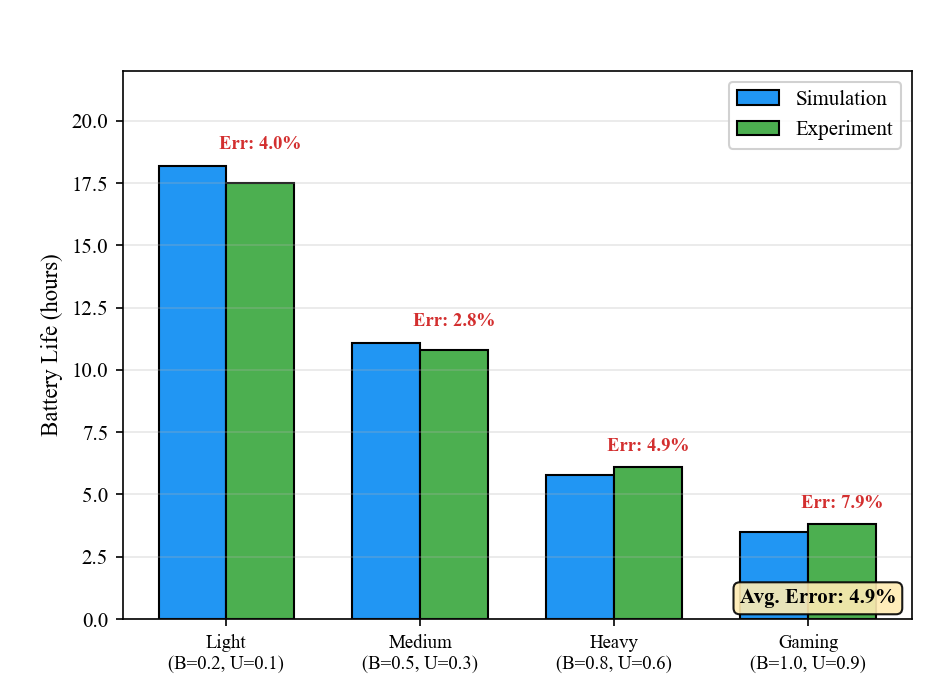
\includegraphics[width=0.85\textwidth]{figures/figure/ABDF6375C82F9A969C2F860CFDC741A7.png}
    \caption{Detailed simulation versus experiment comparison showing battery life (hours) for Light, Medium, Heavy, and Gaming usage scenarios. Error percentages are annotated for each scenario, with the average prediction error of 4.9\% demonstrating strong model accuracy across diverse usage patterns.}
    \label{fig:validation_detailed}
\end{figure}